\documentclass[12pt, titlepage]{article}

\usepackage{booktabs}
\usepackage{graphicx}
\usepackage{tabularx}
\usepackage{hyperref}
\usepackage{mdframed}
\hypersetup{
    colorlinks,
    citecolor=black,
    filecolor=black,
    linkcolor=red,
    urlcolor=blue
}
\usepackage[round]{natbib}


\newmdenv[linecolor=black]{reqbox}

\title{SE 3XA3: Requirements Document\\xPyCharts}

\author{Team 4, xPy
		\\ Hatim Rehman (rehmah3)
		\\ Louis Bursey (burseylj)
		\\ Sarthak Desai (desaisa3)
}

\date{\today}

%% Comments

\usepackage{color}

\newif\ifcomments\commentstrue

\ifcomments
\newcommand{\authornote}[3]{\textcolor{#1}{[#3 ---#2]}}
\newcommand{\todo}[1]{\textcolor{red}{[TODO: #1]}}
\else
\newcommand{\authornote}[3]{}
\newcommand{\todo}[1]{}
\fi

\newcommand{\wss}[1]{\authornote{blue}{SS}{#1}}
\newcommand{\ds}[1]{\authornote{red}{DS}{#1}}
\newcommand{\mj}[1]{\authornote{red}{MSN}{#1}}
\newcommand{\cm}[1]{\authornote{red}{CM}{#1}}
\newcommand{\mh}[1]{\authornote{red}{MH}{#1}}

% team members should be added for each team, like the following
% all comments left by the TAs or the instructor should be addressed
% by a corresponding comment from the Team

\newcommand{\tm}[1]{\authornote{magenta}{Team}{#1}}


\begin{document}

\maketitle

\pagenumbering{roman}
\tableofcontents
\listoftables
\listoffigures

\begin{table}[bp]
\caption{\bf Revision History}
\begin{tabularx}{\textwidth}{p{3cm}p{2cm}X}
\toprule {\bf Date} & {\bf Version} & {\bf Notes}\\
\midrule
Oct. 10, 2016 & 1.0 & Revision 0\\
\bottomrule
\end{tabularx}
\end{table}

\newpage

\pagenumbering{arabic}

This document describes the requirements for XPYCharts, a Python graphing library.  The template for the Software
Requirements Specification (SRS) is a subset of the Volere
template~\citep{RobertsonAndRobertson2012}.  

\section{Project Drivers}

\subsection{The Purpose of the Project}
The project being constructed is a recreation of JCharts, a graphing library available to developers in Java. The purpose of XPYCharts is to allow users to incorporate graphing capabilities into programs and generate simple line graphs in their programs. There are several existing programs that allow graphing on various platforms, such as graphing calculators and online graphing tools, however, graphing libraries are often hard to incorporate into programs. XPYCharts aims to be a simple to use product that can be used to accurately graph data points and produce smooth graphs.

\subsection{The Stakeholders}

\subsubsection{The Client}
The client of the project is a company requiring a graphing library. The company is interested in deploying the graphing library as an educational tool to students and to other end users that may be developers. The client will be the one reviewing all the prototypes of the project and conducting evaluation before the project is deployed into the market.
\subsubsection{The Customers}
The Customers of the project are the end users who will be using the graphing library in their programs. This includes students of computer science in schools who are looking to graph their research work or use graphs within their applications. This group also include developers who require graphs in their applications. Furthermore, data scientists can use this library to enter large datasets in order to study trends and conduct research.
\subsubsection{Other Stakeholders}
Other stakeholders include the developers who are creating the project and who will be responsible for all future updates and maintenance.
\subsection{Mandated Constraints}
\textcolor{red}{Format, add more as well - CM} \\
Description: The User must have Python 2.7 installed on their device.
Rationale: User can only import and use the library inside Python 2.7
Fit Criterion: The library will be able to be imported into Python 100\% of the time if Python 2.7 is installed on the system. If the user doesn't have Python 2.7 a link in the User Manual will lead 	the user to the appropriate download location.

\subsection{Naming Conventions and Terminology}
\begin{center}
\begin{table}[!hpb]
    \caption{Terminology} 
    \begin{tabular}{ |c|p{11cm}|}
	\hline
	Term & Definition\\ \hline
	API & Are routines and protocols that allow software development by specifying how software components should interact with each other.  \\ \hline
	JCharts & The existing graphing library that is being recreated in this project.\\ \hline
	XPYCharts & This is the name of the project/library that is being created.\\ \hline
	Library & Is a collection of already made routines that can be incorporated into a program to enable additional functionalities.\\ \hline
	Client & Is the party that wants the project to be built.The individuals who are the main investors/stakeholders.\\ \hline
	Stakeholders & The individuals/parties that have something to gain/loose from the outcome of the project or someone who is interested/concerned about the outcome of the project.\\ \hline
	MATLAB & A high level language that is used for technical computing, visualization, graphing, and programming practices.\\ \hline
	Python 2.7 & Is a high level programming language. This is language in which the library will be developed and the language for the library will be available for use.\\ \hline
    \end{tabular}
\end{table}
\end{center}
\subsection{Relevant Facts and Assumptions}
\textcolor{red}{Include details about environment and the people using the program - CM} \\
It is assumed here that graphing libraries are a valuable resource in educational, research and development environments and that each party involved will benefit from the production of this software. It is also assumed that the client currently only wants the project to produce line graphs and any further graphing capabilities may or may not be added depending on the client's decision and the time constraints.
\clearpage
\section{Functional Requirements}

\subsection{The Scope of the Work and the Product}

\subsubsection{The Context of the Work}
The context can be seen by the following visual, describing user interaction with the program and program response. \\
		
	\begin{figure}[!htb]
		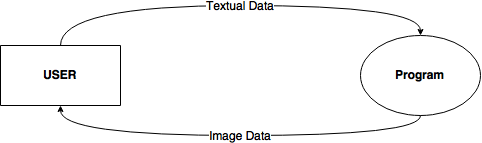
\includegraphics[scale=0.8]{img/ContextDiagram.png}
		\caption{Context Diagram}
	\end{figure}
	
\subsubsection{Work Partitioning}
\textcolor{red}{Include work being done by User and dependant programs. Note what entity is doing what work - CM} \\
\textcolor{red}{Consider more work being done by outside sources by the program, if any exist - CM} \\
\begin{center}
\begin{table}[!hpb]
    \caption{Work Partitioning} 
    \begin{tabular}{ |c|p{11cm}|}
	\hline
	Event No. & Event\\ \hline
	1 & Create the (Cartesian) coordinate system that is centered within a window.\\ \hline
	2 & Add labels to the coordinate system. \\ \hline
	3 & Plot sample points.\\ \hline
	4 & Construct a line that joins two points together.\\ \hline
	5 & Finishing edits (i.e input checking and error handling).\\ \hline
    \end{tabular}

\end{table}
\end{center}

\subsubsection{Individual Product Use Cases}
\textcolor{red}{Different graphs, different export formats... Think of more cases - CM} \\
Because of the nature of the product, a universal use case exists: 

\begin{reqbox}
    \begin{tabular}{l p{10cm}}

	\bf{Use Case \#: 1} & \\
	 & \\
	{\bfseries Scenario: } 	& 	Constructing a graph from a set of data.	\\
	{\bfseries Trigger: }   		& 	User request. 					\\
	{\bfseries Precondition: } 	&	Data inputted in the correct format.		\\
	{\bfseries PostCondition } 	& 	Graph generated and outputted to the user's screen.				\\

    \end{tabular}
\end{reqbox}


\subsection{Functional Requirements}
\textcolor{red}{How will it read data? - CM} \\
\begin{reqbox}
%---
\begin{tabular}{ccc}Requirement \#: 1
\end{tabular} \\
%---
\textbf{Description:} The software shall read data given to it.\\
\textbf{Rationale:} Data is needed to construct a graph. \\
\textbf{Originator:} Hatim Rehman \\
\textbf{Fit Criterion:} The data used by the program is identical to the data given to it.\\
%---
\begin{tabular}{ll}
\textbf{Customer Satisfaction:} 5 & \textbf{Customer Dissatisfaction:} 5 \\
\textbf{Priority:} High & \textbf{Conflicts:} 2,3,4,5\\
\end{tabular} \\
%---  
\textbf{History:} Created October 10, 2016
%--
\end{reqbox}

\begin{reqbox}
%---
\begin{tabular}{ccc}Requirement \#: 2
\end{tabular} \\
%---
\textbf{Description:} The software will raise an exception if the data format cannot be plotted, and stop the program. \\
\textbf{Rationale:} It is safer to stop the program after it is realized the data points do not meet the expected format, versus letting the program proceed to unexpected behaviour. \\
\textbf{Originator:} Hatim Rehman \\
\textbf{Fit Criterion:} The program execution halts when improper data is entered.\\
%---
\begin{tabular}{ll}
\textbf{Customer Satisfaction:} 5 & \textbf{Customer Dissatisfaction:} 5 \\
\textbf{Priority:} High & \textbf{Conflicts:} 3,4,5\\
\end{tabular} \\
%---  
\textbf{History:} Created October 10, 2016
%--
\end{reqbox}

\begin{reqbox}
%---
\begin{tabular}{ccc}Requirement \#: 3
\end{tabular} \\
%---
\textbf{Description:} The software will construct a coordinate system that will fit all the data points.\\
\textbf{Rationale:} This ensures the coordinate system is always dynamically generated to work for all data sets. \\
\textbf{Originator:} Hatim Rehman \\
\textbf{Fit Criterion:} The maximum value on the xy axes is $\geq$ maximum x, y in data set.\\
%---
\begin{tabular}{ll}
\textbf{Customer Satisfaction:} 5 & \textbf{Customer Dissatisfaction:} 5 \\
\textbf{Priority:} High & \textbf{Conflicts:} 4,5\\
\end{tabular} \\
%---  
\textbf{History:} Created October 10, 2016
%--
\end{reqbox}

\begin{reqbox}
%---
\begin{tabular}{ccc}Requirement \#: 4
\end{tabular} \\
%---
\textbf{Description:} The software shall plot all the data points.\\
\textbf{Rationale:} The user will want all the data plotted. \\
\textbf{Originator:} Hatim Rehman \\
\textbf{Fit Criterion:} All data points exist on the generated graph.\\
%---
\begin{tabular}{ll}
\textbf{Customer Satisfaction:} 5 & \textbf{Customer Dissatisfaction:} 5 \\
\textbf{Priority:} High & \textbf{Conflicts:} 5\\
\end{tabular} \\
%---  
\textbf{History:} Created October 10, 2016
%--
\end{reqbox}
\textcolor{red}{Come with a better way to phrase this one - CM} \\
\begin{reqbox}
%---
\begin{tabular}{ccc}Requirement \#: 5
\end{tabular} \\
%---
\textbf{Description:} The software will connect a line that passes through all the data points if the data points are a function of x.\\
\textbf{Rationale:} Imposing a constraint on only graphing functions ensures validity and correctness (a function only has one interpretation), whereas graphing relations introduces ambiguity in the shape of the line. \\
\textbf{Originator:} Hatim Rehman \\
\textbf{Fit Criterion:} A line passes through all the points if there is only one y value for each x.\\
%---
\begin{tabular}{ll}
\textbf{Customer Satisfaction:} 5 & \textbf{Customer Dissatisfaction:} 5 \\
\textbf{Priority:} High & \textbf{Conflicts:} None\\
\end{tabular} \\
%---  
\textbf{History:} Created October 10, 2016
%--
\end{reqbox}
\clearpage

\section{Non-functional Requirements} %Louis

\subsection{Look and Feel Requirements}
%
%-----------Visually appealing
%
\textcolor{red}{On what scale? - CM} \\
\begin{reqbox}
%---
\begin{tabular}{ccc}
Requirement \#: 1& Requirement Type: 10a & Event/Use case \#: \\
\end{tabular} \\
%---
\textbf{Description:} The graphs produced should be visually appealing and look professional \\
\textbf{Rationale:} The programmer may be producing graphs for presentations, and will appreciate a good looking product \\
\textbf{Originator:} Louis Bursey\\
\textbf{Fit Criterion:} 70\% of people surveyed believe that graphs are visually appealing and look professional  \\
%---
\begin{tabular}{ll}
\textbf{Customer Satisfaction:} 4 & \textbf{Customer Dissatisfaction:} 2 \\
\textbf{Priority:} Medium & \textbf{Conflicts:} None\\
\end{tabular} \\
%---  
\textbf{Supporting Materials:} None \\
\textbf{History:} Created October 5, 2016
%--
\end{reqbox}
%
% No style req.
%
\subsection{Usability and Humanity Requirements}

%
%-----------Easy to use
%
\begin{reqbox}
%---
\begin{tabular}{ccc}
Requirement \#: & Requirement Type: 11a & Event/Use case \#: \\
\end{tabular} \\
%---
\textbf{Description:} The product should be easy to use for novice Python programmers \\
\textbf{Rationale:} The programmer using this library should be able to focus on their program, not on using this library \\
\textbf{Originator:} Louis Bursey\\
\textbf{Fit Criterion:} 80\% of programmers familiar with Python successfully use the product  \\
%---
\begin{tabular}{ll}
\textbf{Customer Satisfaction:} 4 & \textbf{Customer Dissatisfaction:} 3 \\
\textbf{Priority:} Medium & \textbf{Conflicts:} None\\
\end{tabular} \\
%---  
\textbf{Supporting Materials:} None \\
\textbf{History:} Created October 5, 2016
%--
\end{reqbox}

%
%-----------Language
%
\begin{reqbox}
%---
\begin{tabular}{ccc}
Requirement \#: & Requirement Type: 11b & Event/Use case \#: \\
\end{tabular} \\
%---
\textbf{Description:} When natural language is required, this product will use English \\
\textbf{Rationale:} Python is written in English \\
\textbf{Originator:} Louis Bursey\\
\textbf{Fit Criterion:}  No non-English natural language is used in the product \\
%---
\begin{tabular}{ll}
\textbf{Customer Satisfaction:} 1 & \textbf{Customer Dissatisfaction:} 5 \\
\textbf{Priority:} High & \textbf{Conflicts:} None\\
\end{tabular} \\
%---  
\textbf{Supporting Materials:} None \\
\textbf{History:} Created October 5, 2016
%--
\end{reqbox}
%
% No personalization unless you mean the actual graphs, I believe that would be a functional requirement?
%
%
%-----------Quick to learn
%
\begin{reqbox}
%---
\begin{tabular}{ccc}
Requirement \#: & Requirement Type: 11c & Event/Use case \#: \\
\end{tabular} \\
%---
\textbf{Description:} The programmer using this product should quickly be able to learn how to use this product \\
\textbf{Rationale:} Programmers who face a steep learning curve will be discouraged from using this product \\
\textbf{Originator:} Louis Bursey\\
\textbf{Fit Criterion:}  Programmers familiar with Python are able to produce graphs within an average twenty minutes of acquiring the library \\
%---
\begin{tabular}{ll}
\textbf{Customer Satisfaction:} 4 & \textbf{Customer Dissatisfaction:} 4 \\
\textbf{Priority:} Medium & \textbf{Conflicts:} None\\
\end{tabular} \\
%---  
\textbf{Supporting Materials:} None \\
\textbf{History:} Created October 5, 2016
\end{reqbox}
%
%-----------Error messages
%
\begin{reqbox}
%---
\begin{tabular}{ccc}
Requirement \#: & Requirement Type: 11d & Event/Use case \#: \\
\end{tabular} \\
%---
\textbf{Description:} When used incorrectly, the product should generate error messages that are easy to understand \\
\textbf{Rationale:} Knowing when and how the library is being used incorrectly will help developers use the library more efficiently. \\
\textbf{Originator:} Louis Bursey\\
\textbf{Fit Criterion:}  80\% of programmers using the library for the first time can understand the error messages they create \\
%---
\begin{tabular}{ll}
\textbf{Customer Satisfaction:} 5 & \textbf{Customer Dissatisfaction:} 4 \\
\textbf{Priority:} High & \textbf{Conflicts:} None\\
\end{tabular} \\
%---  
\textbf{Supporting Materials:} None \\
\textbf{History:} Created October 5, 2016
%--
\end{reqbox}
%
% No accessibility, outside of the scope of this project
%

\subsection{Performance Requirements}
%
%-----------Speed
%
\begin{reqbox}
%---
\begin{tabular}{ccc}
Requirement \#: & Requirement Type: 12a & Event/Use case \#: \\
\end{tabular} \\
%---
\textbf{Description:} The product should generate graphs in a timely manner \\
\textbf{Rationale:} The program should not take so long that it slows down the programmer's workflow \\
\textbf{Originator:} Louis Bursey\\
\textbf{Fit Criterion:}  The library takes under 20 seconds to generate graphs of a reasonable size \\
%---
\begin{tabular}{ll}
\textbf{Customer Satisfaction:} 4 & \textbf{Customer Dissatisfaction:} 4 \\
\textbf{Priority:} High & \textbf{Conflicts:} None\\
\end{tabular} \\
%---  
\textbf{Supporting Materials:} None \\
\textbf{History:} Created October 5, 2016
%--
\end{reqbox}
%
% No safety critical requirements
%

%
%-----------Precision                                                     %confirm on precision
%
\begin{reqbox}
%---
\begin{tabular}{ccc}
Requirement \#: & Requirement Type: 12c & Event/Use case \#: \\
\end{tabular} \\
%---
\textbf{Description:} The product should produce accurate graphs \\
\textbf{Rationale:} Visual representations of data are useless if they don't represent data faithfully \\
\textbf{Originator:} Louis Bursey\\
\textbf{Fit Criterion:}  Graphs produced should have no less than 20\% difference between it and a graph generated by JCharts  \\
%---
\begin{tabular}{ll}
\textbf{Customer Satisfaction:} 5 & \textbf{Customer Dissatisfaction:} 5 \\
\textbf{Priority:} High & \textbf{Conflicts:} None\\
\end{tabular} \\
%---  
\textbf{Supporting Materials:} None \\
\textbf{History:} Created October 5, 2016
%--
\end{reqbox}
%
%-----------Reliability
%
\begin{reqbox}
%---
\begin{tabular}{ccc}
Requirement \#: & Requirement Type: 12d & Event/Use case \#: \\
\end{tabular} \\
%---
\textbf{Description:} The product should always be available \\
\textbf{Rationale:} The product cannot unexpectedly go out of service, as programmers will depend on its availability \\
\textbf{Originator:} Louis Bursey\\
\textbf{Fit Criterion:}  The product is always available  \\
%---
\begin{tabular}{ll}
\textbf{Customer Satisfaction:} 1 & \textbf{Customer Dissatisfaction:} 5 \\
\textbf{Priority:} High & \textbf{Conflicts:} None\\
\end{tabular} \\
%---  
\textbf{Supporting Materials:} None \\
\textbf{History:} Created October 5, 2016
%--
\end{reqbox}
%
%-----------Robustness
%
\begin{reqbox}
%---
\begin{tabular}{ccc}
Requirement \#: & Requirement Type: 12e & Event/Use case \#: \\
\end{tabular} \\
%---
\textbf{Description:} The library will not stall out, if used incorrectly it will always display error messages and abort\\
\textbf{Rationale:} Programmers using the library will depend on graphs not stalling out their programs \\
\textbf{Originator:} Louis Bursey\\
\textbf{Fit Criterion:}    Errors in use always create error messages and aborts, not stalls\\
%---
\begin{tabular}{ll}
\textbf{Customer Satisfaction:} 1 & \textbf{Customer Dissatisfaction:} 5 \\
\textbf{Priority:} High & \textbf{Conflicts:} None\\
\end{tabular} \\
%---  
\textbf{Supporting Materials:} None \\
\textbf{History:} Created October 5, 2016
%--
\end{reqbox}
%
%-----------Capacity                     %%%confirm on graph size
%
\begin{reqbox}
%---
\begin{tabular}{ccc}
Requirement \#: & Requirement Type: 12f & Event/Use case \#: \\
\end{tabular} \\
%---
\textbf{Description:} The library will be able to produce graphs with up to 500 data points \\
\textbf{Rationale:} Programmers using the library will want to build graphs from large data sets \\
\textbf{Originator:} Louis Bursey\\
\textbf{Fit Criterion:}  Graph with up to 500 data points can be generated without problems\\
%---
\begin{tabular}{ll}
\textbf{Customer Satisfaction:} 3 & \textbf{Customer Dissatisfaction:} 5 \\
\textbf{Priority:} High & \textbf{Conflicts:} None\\
\end{tabular} \\
%---  
\textbf{Supporting Materials:} None \\
\textbf{History:} Created October 5, 2016
%--
\end{reqbox}
%
% No scalability
%
% No longevity
%
\subsection{Operational and Environmental Requirements}

%
%-----------Environment---PCs                 
%
\begin{reqbox}
%---
\begin{tabular}{ccc}
Requirement \#: & Requirement Type: 13a & Event/Use case \#: \\
\end{tabular} \\
%---
\textbf{Description:} The product should operate on laptops and desktops \\
\textbf{Rationale:} Programmers work on laptops and desktops and the library should work in this environment \\
\textbf{Originator:} Louis Bursey\\
\textbf{Fit Criterion:}  Personal computer users can run programs that use the library\\
%---
\begin{tabular}{ll}
\textbf{Customer Satisfaction:} 3 & \textbf{Customer Dissatisfaction:} 5 \\
\textbf{Priority:} High & \textbf{Conflicts:} None\\
\end{tabular} \\
%---  
\textbf{Supporting Materials:} None \\
\textbf{History:} Created October 5, 2016
%--
\end{reqbox}

%
%-----------Environment---Python                     
%
\begin{reqbox}
%---
\begin{tabular}{ccc}
Requirement \#: & Requirement Type: 13a & Event/Use case \#: \\
\end{tabular} \\
%---
\textbf{Description:} The product should be usable as a Pyton library \\
\textbf{Rationale:} The Python language is the supported language of this project\\
\textbf{Originator:} Louis Bursey\\
\textbf{Fit Criterion:}  The product is importable in a Python program\\
%---
\begin{tabular}{ll}
\textbf{Customer Satisfaction:} 1 & \textbf{Customer Dissatisfaction:} 5 \\
\textbf{Priority:} High & \textbf{Conflicts:} None\\
\end{tabular} \\
%---  
\textbf{Supporting Materials:} None \\
\textbf{History:} Created October 5, 2016
%--
\end{reqbox}
%
%
% Don't think it needs to interface, confirm?
%
%
%-----------Productization
%
\begin{reqbox}
%---
\begin{tabular}{ccc}
Requirement \#: & Requirement Type: 13c & Event/Use case \#: \\
\end{tabular} \\
%---
\textbf{Description:} \\
\textbf{Rationale:} The product should be distributed as a zip file that is importable in Python programs\\
\textbf{Originator:} Louis Bursey\\
\textbf{Fit Criterion:}  The product is importable in a Python program\\
%---
\begin{tabular}{ll}
\textbf{Customer Satisfaction:} 3 & \textbf{Customer Dissatisfaction:} 4 \\
\textbf{Priority:} High & \textbf{Conflicts:} None\\
\end{tabular} \\
%---  
\textbf{Supporting Materials:} None \\
\textbf{History:} Created October 5, 2016
%--
\end{reqbox}

%
%-----------Release
%
\begin{reqbox}
%---
\begin{tabular}{ccc}
Requirement \#: & Requirement Type: 13d & Event/Use case \#: \\
\end{tabular} \\
%---
\textbf{Description:}Future releases of the project will be backwards compatible \\
\textbf{Rationale:} Backwards compatibility keeps programmers from having to update their code when we make changes\\
\textbf{Originator:} Louis Bursey\\
\textbf{Fit Criterion:}  Releases are backwards compatible\\
%---
\begin{tabular}{ll}
\textbf{Customer Satisfaction:} 2 & \textbf{Customer Dissatisfaction:} 5 \\
\textbf{Priority:} High & \textbf{Conflicts:} None\\
\end{tabular} \\
%---  
\textbf{Supporting Materials:} None \\
\textbf{History:} Created October 5, 2016
%--
\end{reqbox}

\subsection{Maintainability and Support Requirements}
%
% no maintenance requirements for this project
%
% No support requirements for this project
%
%
%-----------Adaptability to OS's
%
\begin{reqbox}
%---
\begin{tabular}{ccc}
Requirement \#: & Requirement Type: 13d & Event/Use case \#: \\
\end{tabular} \\
%---
\textbf{Description:}The product should work in Windows, Linux and Mac OSX environments \\
\textbf{Rationale:} Programmers working in all of these environments will need graphing capabilities\\
\textbf{Originator:} Louis Bursey\\
\textbf{Fit Criterion:}  The library is usable in all of these environments \\
%---
\begin{tabular}{ll}
\textbf{Customer Satisfaction:} 4 & \textbf{Customer Dissatisfaction:} 5 \\
\textbf{Priority:} High & \textbf{Conflicts:} None\\
\end{tabular} \\
%---  
\textbf{Supporting Materials:} None \\
\textbf{History:} Created October 5, 2016
%--
\end{reqbox}


\subsection{Security Requirements}
There are no security requirements for this project
\subsection{Cultural Requirements}
There are no cultural requirements for this project
\subsection{Legal Requirements}
There are no legal requirements for this project
\subsection{Health and Safety Requirements} %end Louis
\textcolor{red}{Note use cases where this may pose a health risk - CM} \\
A graphing library does not pose any serious health and safety risks.

\clearpage
\section{Project Issues}

\subsection{Open Issues}
The major issue currently under investigation is of testing. Although manual testing of the graphs created by the library will be relatively easy to check against existing implementations of graphing libraries and calculators, automated testing is a challenge. The problem exists that there is no existing solution that the team has agreed upon as to how to check graphs that are generated during automatic testing. One solution that was initially suggested was to export the graph generated by the library as a JPEG file and compare it against another image file created by an existing implementation. However, variances in the scales or the differences in the formatting of the two graphs can lead to inaccurate outcomes to the image comparisons. The team is actively looking to solve this issue. 
\subsection{Off-the-Shelf Solutions}
Existing off the shelf solutions include the Jchart Library that is currently available for Java on multiple platforms such as Mac and Windows. MATLAB is another widely known solution often used by students and professionals. There are also Python developed online graphing technologies such as Plotty. The team will be further looking into each of these existing products in order to gather information and for guidance on the project. 
\subsection{New Problems}
There are no new problems that have been encountered by the team.
\newpage
\subsection{Tasks} 
\begin{center}
\begin{table}[!hpb]
    \caption{Tasks} 
    \begin{tabular}{|c|c|}
	\hline
	Tasks & Completion Date \\ \hline
	Develop skeleton axes  & 10/10/16 \\ \hline
	Add axes numbering/Scaling capabilities & 10/14/16 \\ \hline
	Plotting basic (x,y) coordinates & 10/20/16 \\ \hline
	Generate lines to connect plotted data points & 10/28/16 \\ \hline
	Implement smooth curves for connecting data points & 11/4/16 \\ \hline
	Product release/ Final Client Demonstration  & 11/28/16 \\ \hline
    \end{tabular}
\end{table}
\end{center}
Development Phases (Note: Highlights the major milestones for the project development)\\ \\
Phase 1: Developing the basic output window once the user enters in the information is the first thing that the program must be able to do. This window should display a simple x and y axis. At this point no numbering or labels are required. \\ \\
Phase 2: The program will implement the axes numbering and add the functionality of allowing the users to label axes, titles, change scales (more customizable).\\ \\
Phase 3: In this phase the library should be able to be used to plot multiple points onto the generated graph.\\ \\
Phase 4: The graphs in this phase should include lines that are connecting the data points together. Although the lines may not necessarily be smooth curves.\\ \\
Phase 5: The library should be able to create smooth graphs with curved lines that connect data points. This is an important phase because if the library's functional requirements are changed to include graphing different types of functions then smooth curves will be required to properly depict functions.\\ \\
Phase 6: By this point all final changes should be made and the product should be ready to be deployed to end users.\\ \\
Note: Throughout all these phases of development testing will be a reoccurring phase. Testing will be done through both manual and automated methods. However, currently automated testing is still an open issue. \\ \\

\subsection{Migration to the New Product}
Migration will not be an issue in this project. The library will be created for Python 2.7 only. The project will not pursue migration to Python 3.
\subsection{Risks}
There are existing risks regarding the scaling and intervals of the data points, given that the project has currently set up to 500 data points as a upper limit to accurate functionality. Given that a user has a larger amount of data points that need plotting the program may not allow to do so without compromising the non functional requirement of generating graphs in reasonable timings. However, if the program is completely limited to only allowing users to enter a certain number of data points the users may yield inaccurate results in terms of data analysis if they can only input partial data.
\subsection{Costs}
\textcolor{red}{Defend further with respect to hosting, delivery, ... etc. - CM} \\
There are no monetary costs associated with the project. All software being used is accessible for free.
\subsection{User Documentation and Training}
The user document will have two major components to support the user. The first document will provide users with a guide on how to unpack the library provided as an archived file and import it correctly into their workspace. The second document will be an API specification documentation that will provide support for the developers allowing them to quickly and efficiently incorporate the library functionalities into their program.
\bibliographystyle{plainnat}

\bibliography{SRS}

\newpage

%\section{Appendix}
%
%This section has been added to the Volere template.  This is where you can place
%additional information.

%\subsection{Symbolic Parameters}
%
%The definition of the requirements will likely call for SYMBOLIC\_CONSTANTS.
%Their values are defined in this section for easy maintenance.

\subsection{Gantt Chart}

The schedule of the project is shown by the following
 \href{run:../DevelopmentPlan/GanttChart.gan} {\underline{Gantt Chart}}.

\end{document}